\subsubsection{13.12.14 (Competition)}
\begin{center}
	1-nd day of competition "Robofest-Ryazan"
\end{center}
Today there were training day.
Improvements that were done:
\begin{enumerate}
	\item MOB was moved to the previous position. 
	
		\begin{figure}[H]
			\begin{minipage}[h]{0.2\linewidth}
				\center  
			\end{minipage}
			\begin{minipage}[h]{0.6\linewidth}
				\center{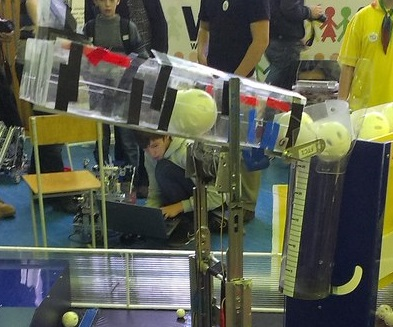
\includegraphics[scale=0.4]{days/13.12.14/images/01}}
				\caption{Mount of MOB (on the robot put the balls into 120cm goal)}
			\end{minipage}
		\end{figure}
	\item It was turned out that bucket can't pass between the slats. So it was cut.
	
		\begin{figure}[H]
			\begin{minipage}[h]{0.2\linewidth}
				\center  
			\end{minipage}
			\begin{minipage}[h]{0.6\linewidth}
				\center{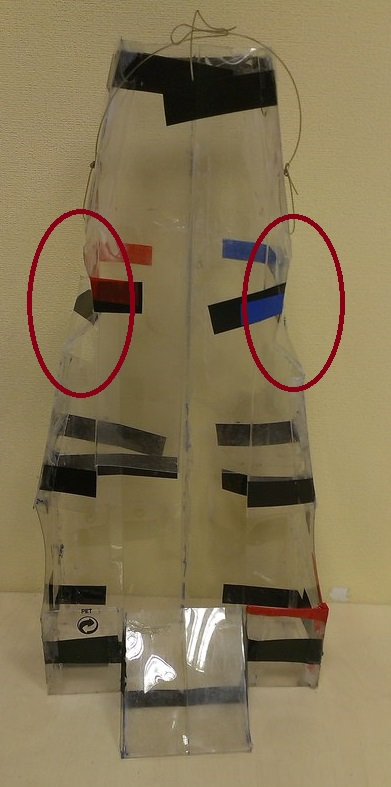
\includegraphics[scale=0.25]{days/13.12.14/images/02}}
				\caption{Bucket was cut}
			\end{minipage}
		\end{figure}
	
	\item It was installed screw that stops the blades of gripper for increase quality capturing small balls. So that blades sharply turns and due to elastic force of blades ball gets into the bucket.
	\begin{figure}[H]
		\begin{minipage}[h]{0.2\linewidth}
			\center  
		\end{minipage}
		\begin{minipage}[h]{0.6\linewidth}
			\center{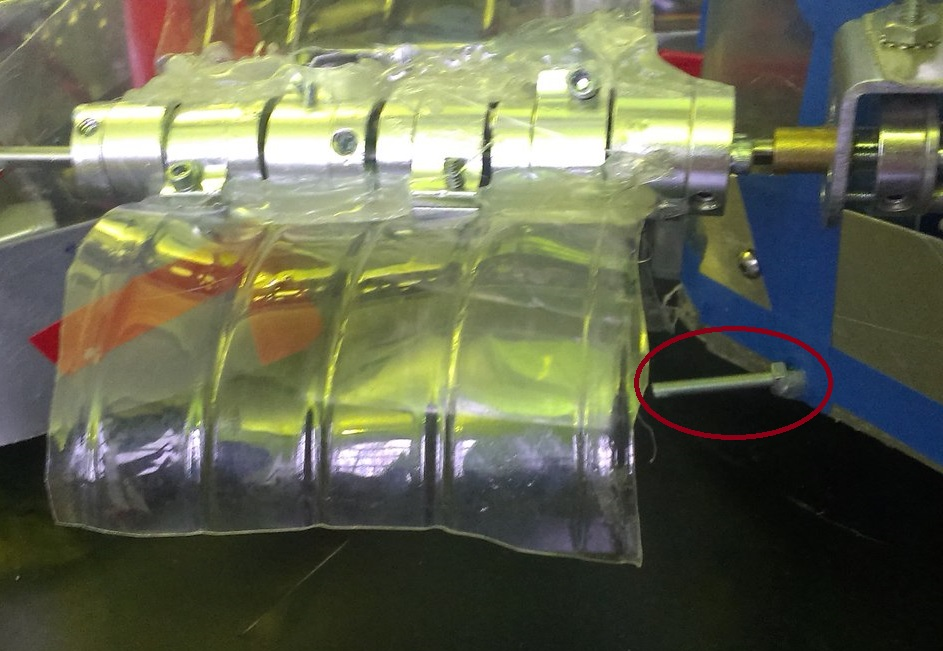
\includegraphics[scale=0.2]{days/13.12.14/images/03}}
			\caption{Screw}
		\end{minipage}
	\end{figure}	
	
	
	\item It was installed mechanism that directs balls vertically.
	
		\begin{figure}[H]
			\begin{minipage}[h]{0.31\linewidth}
				\center{
\includegraphics[scale=0.22]{days/13.12.14/images/04}}
			\end{minipage}
			\hfill
			\begin{minipage}[h]{0.31\linewidth}
				\center{
\includegraphics[scale=0.33]{days/13.12.14/images/05}}
			\end{minipage}
			\hfill
			\begin{minipage}[h]{0.31\linewidth}
				\center{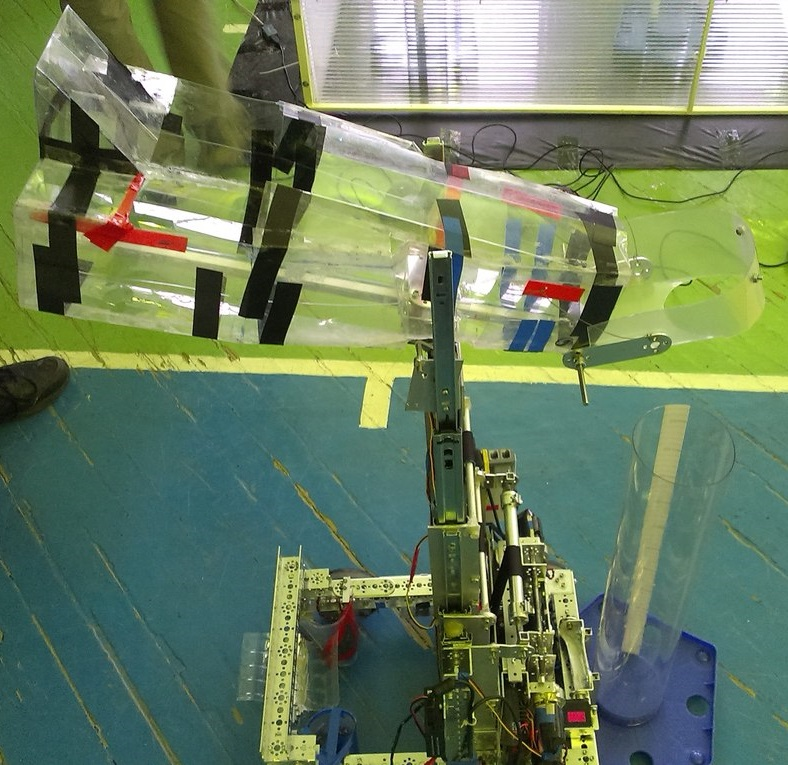
\includegraphics[scale=0.2]{days/13.12.14/images/06}}
			\end{minipage}
			\caption{Mechanism that directs balls vertically}
		\end{figure}
	
	\item During the trainings mount of one axis was broke. It happend due to that the axis was fixed too close to edge of the plate. So the axis was moved.
	
		\begin{figure}[H]
			\begin{minipage}[h]{0.2\linewidth}
				\center  
			\end{minipage}
			\begin{minipage}[h]{0.6\linewidth}
				\center{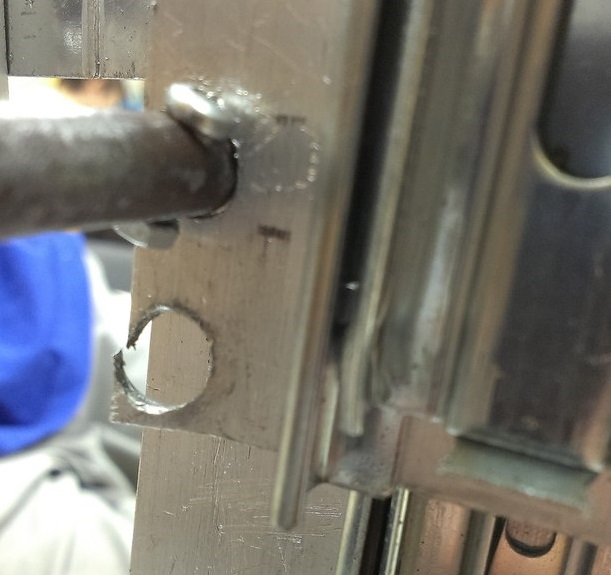
\includegraphics[scale=0.25]{days/13.12.14/images/07}}
				\caption{Broken mount for axis}
			\end{minipage}
		\end{figure}
		
	\item All slats were oiled.	
	
	\item They were installed slopes that prevents balls stuck on the front motors. They were not closed from the top. We think that it's not a problem because the slopes has enough heigh and balls can't to stuck on the motor. 
	
    \item Programme of autonomous period was corrected in accordance with friction on this field.
	
\end{enumerate}
\fillpage